\documentclass[11pt]{article}
\usepackage{times}
\usepackage{ifthen}
\usepackage[dvips]{graphics}
\usepackage[dvips]{color}
\usepackage{epsfig}
%\usepackage{subfigure}
\usepackage[dvips,colorlinks,bookmarks,pdfpagemode=UseOutlines,linkcolor=blue,pagecolor=blue,urlcolor=blue,letterpaper]{hyperref}
\begin{document}
% File giving definitions of commands and environments.
% Because of a latex bug with counters, this has to be included
% using \input not \include.

%--------------------------------------------------------------------------
% For the set of reals and integers
\newcommand{\rr}{\set{Reals}}
\newcommand{\ii}{\set{Integers}}
\newcommand{\cc}{\set{Complex}}
\newcommand{\nn}{\set{Naturals}}

%--------------------------------------------------------------------------
% For figure captions.
% Puts them in sanserif font, indented on both sides.
%   arg: The caption.
\newcommand{\figcaption}[1]{\textsf{\begin{center}\begin{minipage}{5in}
\caption{#1}
\end{minipage}\end{center}}}

%--------------------------------------------------------------------------
% For terms being defined.
% Puts them in bold face and creates an index entry.
%   arg: The term being defined.
% NOTE: To get boldface in the index, do |textbf after #1.
% But this breaks hyperlinks.
\newcommand{\defn}[1]{\textbf{#1}\index{#1}}

%--------------------------------------------------------------------------
% For terms being indexed.
% Puts them in standard font face and creates an index entry.
%   arg: The term being defined.
\newcommand{\pointer}[1]{#1\index{#1}}

%--------------------------------------------------------------------------
% For bold terms to be index, but defined elsewhere
% Puts them in bold face and creates an index entry.
%   arg: The term being defined.
\newcommand{\strong}[1]{\textbf{#1}\index{#1}}

%--------------------------------------------------------------------------
% For terms to be index, but defined elsewhere
% Puts them in normal face and creates an index entry.
%   arg: The term being defined.
\newcommand{\idx}[1]{#1\index{#1}}

%--------------------------------------------------------------------------
% For set names.
% Puts them in italics. In math mode, yields decent spacing.
%   arg: The name of the set.
\newcommand{\set}[1]{\mbox{\textit{#1}}}

%--------------------------------------------------------------------------
% For real part.
%   arg: The argument of the real part.
\newcommand{\re}[1]{\mbox{\textit{Re}}\{#1\}}

%--------------------------------------------------------------------------
% For imaginary part.
%   arg: The argument of the imaginary part.
\newcommand{\im}[1]{\mbox{\textit{Im}}\{#1\}}

%--------------------------------------------------------------------------
% For matlab commands
%   arg: The name of the command
\newcommand{\matlab}[1]{\texttt{#1}\index{#1 command in Matlab}\index{Matlab!#1}}
\newcommand{\simulink}[1]{\texttt{#1}\index{#1 in Simulink}\index{Simulink!#1}}
\newcommand{\matlabInCaption}[1]{\texttt{#1}}

%--------------------------------------------------------------------------
% For "Probing Further" sidebars.
% Puts them in a floating frame.  It is up to you to ensure that the
% frame fits on one page.
%   arg: the title.
\newenvironment{further}[1]{
\begin{table}[btp]
\centering
\begin{tabular}{|p{5in}|}
\hline
\cr
\begin{minipage} {5in}
\parskip        0.1in
\parindent      0.0in
\subsection* {Probing further: #1}
\addcontentsline{toc}{subsection}{Probing further: #1}
} {
\end{minipage}\cr
\cr
\hline
\end{tabular}
\end{table}
}

%--------------------------------------------------------------------------
% For "Basics" sidebars.
% Puts them in a floating frame.  It is up to you to ensure that the
% frame fits on one page.
%   arg: the title.
\newenvironment{basics}[1]{
\begin{table}[btp]
\centering
\begin{tabular}{|p{5in}|}
\hline
\cr
\begin{minipage} {5in}
\parskip        0.1in
\parindent      0.0in
\subsection* {Basics: #1}
\addcontentsline{toc}{subsection}{Basics: #1}
} {
\end{minipage}\cr
\cr
\hline
\end{tabular}
\end{table}
}

%--------------------------------------------------------------------------
% For "Tips and Tricks" sidebars.
% Puts them in a floating frame.  It is up to you to ensure that the
% frame fits on one page.
%   arg: the title.
\newenvironment{tricks}[1]{
\begin{table}[btp]
\centering
\begin{tabular}{|p{5in}|}
\hline
\cr
\begin{minipage} {5in}
\parskip        0.1in
\parindent      0.0in
\subsection* {Tips and Tricks: #1}
\addcontentsline{toc}{subsection}{Tips and Tricks: #1}
} {
\end{minipage}\cr
\cr
\hline
\end{tabular}
\end{table}
}

%--------------------------------------------------------------------------
% For text that is boxed for emphasis.
\newenvironment{boxed}{
\begin{center}
\begin{tabular}{|p{5in}|}
\hline
\cr
\begin{minipage} {5in}
\parskip        0.1in
\parindent      0.0in
} {
\end{minipage}\cr
\cr
\hline
\end{tabular}
\end{center}
}

%--------------------------------------------------------------------------
% For examples
% NOTE: Because of this line, this has to be included using \input
% not \include.
\newcounter{example}
\newenvironment{example}{
\refstepcounter{example}
\begin{quote}
\textbf{Example \arabic{chapter}.\arabic{example}:}
} {
\end{quote}
}
\renewcommand \theexample {\thechapter.\arabic{example}}


\title{Technical Specification for Soft Walls -
Flight Control Systems to Limit the Flight Space of Commercial Aircraft}
\author{Edward A. Lee, Xiaojun Liu, and J. Adam Cataldo\\
eal@eecs.berkeley.edu, liuxj@eecs.berkeley.edu, acataldo@eecs.berkeley.edu\\
Electrical Engineering \& Computer Science\\
University of California, Berkeley}
\date{11 February 2002}

\maketitle

\section{Introduction}

See the companion document that discusses the issue.

\section{Two-Dimensional Model}

\subsection{Two-Dimensional Aircraft Model}

We consider first a two-dimensional model that addresses
control of the heading of an aircraft.
Let the position of the aircraft be a function
\[
p \colon \rr \to \rr ^2
\]
where the domain is
time (the reals) and the range is the position of the aircraft
in two-dimensional space.
Let $\dot{p}$ denote the derivative with respect to time (the
velocity) and $\ddot{p}$ the second derivative with respect to time (the
acceleration). Let $p_x$ denote the position in the $x$ direction (east-west,
increasing to the east), and let $p_y$ denote the position in the $y$ direction
(north-south, increasing to the north). Similarly, $\dot{p_x}$ and $\ddot{p_x}$
denote the speed and acceleration in the $x$ direction (east).

Let the speed $s$ of the aircraft be given by
\[
\forall ~ t \in \rr, \quad
s(t) = |\dot{p}(t)| .
\]
Let
\[
\theta \colon \rr \to [-\pi, \pi)
\]
be the heading of the aircraft, where 0 is due east, so that
\[
\forall ~ t \in \rr, \quad
\dot{p} (t) = (s(t) \cos(\theta (t)), s(t) \sin(\theta(t))) .
\]

Assume that under normal circumstances, the pilot controls the rate of
change of heading, $\dot{\theta}$, through a combination of differential
thrust on the engines and movement of the rudder and other control
surfaces. Moreover, the pilot controls the speed via overall thrust
(and vertical movement, which we are not yet considering).
Thus, the inputs to the aircraft model are $\dot{\theta}$ and $s$.

\begin{figure}[btp]
\centering
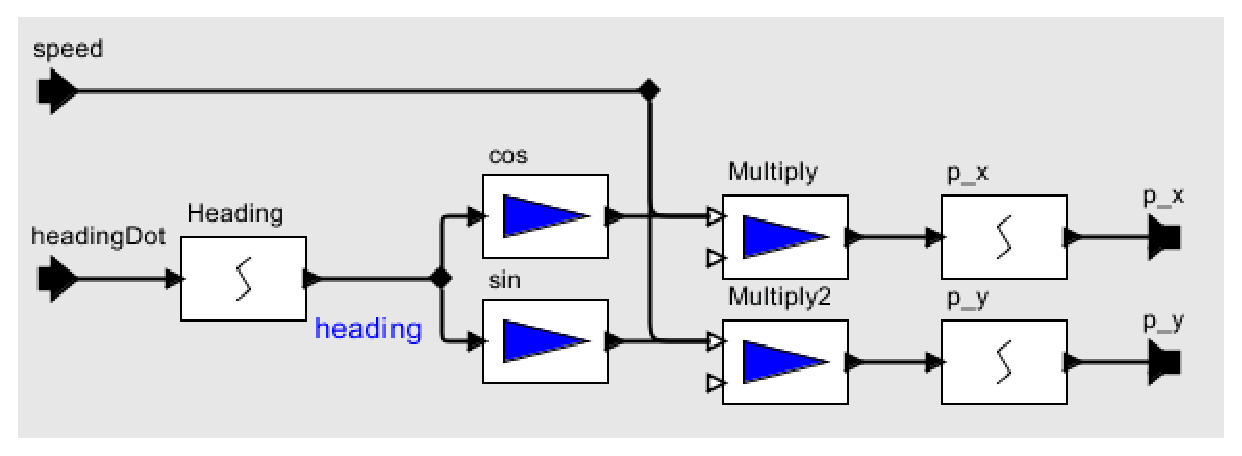
\includegraphics[width=5in]{fig2Daircraft.eps}
\figcaption{Two dimensional aircraft model.
\label{fig2Daircraft}}
\end{figure}

The two dimensional model for the aircraft is shown in figure
\ref{fig2Daircraft}.

\subsection{Turn Radius}

Assume the speed is a constant $s$, so the pilot controls only heading.
Then the turning radius is
\[
r = s/\dot{\theta} .
\]
To see this, assume the rate of change of heading is a constant,
$\dot{\theta} = \alpha$. Assume that $\alpha$ is given in radians/second and
$s$ in meters per second.  It takes $\tau = 2 \pi /\alpha$ seconds
to complete one circle.  Upon completing the circle, the aircraft
will have covered a distance of $s\tau = 2 \pi s/\alpha$ meters.
Since the radius of a circle times $2 \pi$ is its circumference,
the result follows.

The rate of change of heading as a function of speed and steering
angle is
\[
\dot{\theta} = s/r.
\]
If we assume that the minimum safe turning radius is $r_{min}$, then
the control signal $\dot{\theta}$ must be kept in the range
$[-s/r_{min}, s/r_{min}]$.

For example, if we assume an aircraft traveling at
\[
s = 500~ kilometers/hour
\]
or about 139 meters/second, and we assume the aircraft has a minimum
safe turning radius of $r_{min} = 1000$
meters, then $\dot{\theta}$ must be constrained
to lie in the range $[-0.139, 0.139]$ radians per second.

\subsection{Blending Controller}

Let the pilot's control be $\dot{\theta}_p$ and the control signal
generated by the softwalls system be $\dot{\theta}_s$.
We take the rate of change of heading of the aircraft to
be
\[
\dot{\theta} = \set{limit}_{[-s/r_{min}, s/r_{min}]}
(\dot{\theta}_p - \dot{\theta}_s ),
\]
where $\set{limit}_{[a,b]}$ is a function
\[
\set{limit}_{[a,b]} \colon \rr \to [a, b]
\]
where
\[
\forall ~ u \in \rr, \quad
\set{limit}_{[a,b]}(u) = \left \{
\begin{array}{ll}
b&\mbox{ if } u > b\\
a&\mbox{ if } u < a\\
u&\mbox{ otherwise }
\end{array}
\right .
\]
This strategy for blending the softwalls controller and the
pilot's control ensures that while the control parameter is within
safe limits, the responsivity of the aircraft to the pilot
commands remains normal.
That is, the pilot's control signal is not attenuated.

\subsection{Maintaining Responsivity}

Figure A illustrates how the blending controller maintains responsivity while
biasing the pilot control. When there is no bias, the aircraft will turn as the
pilot intends. When there is a bias of $M$ ($= s/r_{min}$, the maximum rate of
change in heading) to the right, the pilot will not be able to make the
aircraft turn left -- the aircraft will keep straight as the pilot tries to
turn the rudder to the left extreme position.
When the bias increases to $3M/2$ to the right, the aircraft will turn right at
a rate of at least $M/2$, whatever the pilot tries to do.

\section{Softwall Controller -- A First Design}

Here we present our first attempt at designing a softwall controller.
Although later analysis and simulation showed that a malicious pilot can defeat
the controller, the design illuminated the importance of criticality measures
and inspired our criticality-based controller design.

\subsection{Softwall Controll Signal}

Assume a single, flat soft wall with thickness $d_s$.
The \textit{inner boundary} delineates the no-fly zone.
The \textit{outer boundary} delineates the region where the
softwall controller starts to have some effect.
The thickness $d_s$ is the distance between these two boundaries.
Let the distance of the aircraft from the inner boundary of
the soft wall be given by
\[
d \colon \rr \to \rr .
\]
Define the \textit{criticality} to be
\[
c = \set{limit}_{[0,1]}(1 - {{d - r_{min}}\over{d_s - r_{min}}}) .
\]
If the aircraft is further than $d_s$ from the inner boundary of the
softwall, then $c = 0$, indicating that no corrective action is necessary.
If the aircraft is closer than $r_{min}$ to the inner boundary of the softwall,
then $c = 1$, indicating that maximum corrective action is necessary.
If the aircraft is in between these two boundaries, then the criticality
is between 0 and 1.

Let the angle of approach of the aircraft from the soft wall be given by
\[
\theta \colon \rr \to [-\pi, \pi].
\]
We set the corrective control signal to
\[
\dot{\theta}_s = \left \{
\begin{array}{ll}
2 \cos(\theta) c s/r_{min}& \mbox{ if } -\pi / 2 < \theta < \pi / 2 \\
0 & \mbox{ otherwise}
\end{array}
\right .
\]
This results in zero corrective control if the aircraft is moving
away from the wall or parallel to the wall, and maximum corrective
control if the aircraft is approaching head on ($\theta = 0$).  
The single point
of maximum corrective control is when the aircraft is approaching
the wall head on and has distance $r_{min}$ from the inner boundary.
At this point, the corrective control is twice that required to
execute a minimum radius turn.  It is twice that control so that
when added to the pilot's control we are assured of having
the maximum turning control, even if the pilot is maximally
uncooperative in attempting to counteract the control.

\subsection{Resistant Pilot}

We were able to develop a malicious-pilot strategy that, even with the
control scheme of the previous section, can fly the plane into the no-fly zone.
This section explains why the strategy was successful.

The resistant pilot is initially heading towards the no-fly zone, so
the initial $\dot{\theta_{p}}$ is $0$.  That is, the pilot intends to
maintain forward motion and crash into the wall.

Since, before saturation, the input control is $\dot{\theta} =
\dot{\theta_{p}} - \dot{\theta_{s}}$, the pilot will try to counteract
the control signal by chosing $\dot{\theta_{p}} = \dot{\theta_{s}}$.
In a cockpit, the pilot would be physically limited by a maximum
$\dot{\theta_{p}}$, so the pilot uses
\[
\dot{\theta_{p}} = \set{limit}_{[-s/r_{min},s/r_{min}]}(\dot{\theta_{s}})
\]
Here the limit values are chosen for a pilot that would never move the
plane in an unsafe position.  In practice these limit points could be
larger.

\subsection{Boundary Penetration}

The resistant pilot succeeds in penetrating the no-fly zone boundray.
Even though the plane's trajectory is changed, the $\cos{\!(\theta})$ factor
in the corrective control signal dampens the strength of the softwalls
control signal, such that the pilot can fly into the softwall at a
$\pi/6$ angle from the wall.

If the $\cos{\!(\theta)}$ factor is removed from the control signal, this
problem disapears.  That is,
\[
\dot{\theta}_s = \left \{
\begin{array}{ll}
2 c s/r_{min}& \mbox{ if } -\pi / 2 < \theta < \pi / 2 \\
0 & \mbox{ otherwise}
\end{array}
\right .
\]
This control scheme is more restrictive however, because a plane
cannot stay in the softwall.  Any pilot between the inner and outer
boundary will eventually be forced outside the outer boundary, so this
motivated an alternative approach (described in the next section).

\section{Criticality-Based Control}

A measure of criticality assesses the level of threat that an aircraft poses to
a no-fly zone. A general design pattern for softwall controllers is to let their
bias vary with respect to an appropriate criticality measure.

\subsection{A Measure of Criticality}

Here we propose a criticality measure based on how long it will take the plane
to reach the no-fly zone in the worst case. Figure B illustrates this measure.
In this figure, the black dots represent the position of an aircraft, and the
arrows represent its heading. The worst case trajectories are shown as dotted
lines.

Suppose the no-fly zone is defined by $\{(x,y)|\ x \geq b_{x}\}$. The 
criticality measure does not depend on the aircraft's $y$-position. The
equations for calculating $c(x, \theta)$ are:
\[
c(x, \theta) = \left\{ \begin{array}{ll}
\frac{\theta}{M} + \frac{d - r_{min}\sin{\theta}}{s} & \mbox{if $d \geq r_{min}\sin{\theta},\ 0 \leq \theta \leq \pi/2$} \\
\frac{\theta - \arcsin{\left( \frac{r_{min}\sin{\theta}- d}{r_{min}}\right) }}{M} & \mbox{if $d < r_{min}\sin{\theta},\ 0 \leq \theta \leq \pi/2$} \\
\frac{2(\theta - \pi/2)}{M} + c(x, \pi - \theta) & \mbox{if $\pi/2 < \theta \leq \pi$} \\
c(x, |\theta|) & \mbox{if $-\pi \leq \theta < 0$}
\end{array}
\right.
\]
where $d = d_{x} - x$ is the distance between the aircraft and the no-fly zone.
Note that $s$, $r_{min}$, and $M$ are related by $M = s/r_{min}$.

\subsection{Criticality-Based Softwall Controller}

The bias produced by a proposed criticality-based controller is shown in figure
D. The threshold $\pi/M$ is the value of $c(x, \theta)$ when $x = b_{x}$ (the 
aircraft is on the boundary of the no-fly zone), and $\theta = \pi$ (the 
aircraft is flying straight out of the no-fly zone). No bias is needed here.
The threshold $2/M$ is equal to $c(b_{x}-2r_{min}, 0)$ -- the aircraft is flying
head on to the no-fly zone, at a distance of $2r_{min}$ from the zone.
The aircraft can still be safely turned away at half the 
maximum turning rate. Note that the bias level is at $3M/2$, so the plane will
be turned at a rate of at least half the maximum, whatever the pilot tries to
do. The sign (plus -- left, minus -- right) of the bias is chosen to be the
same as $\theta$.

\subsection{Simulation Results}

The model shown in figure (Simulation Model) is constructed in Ptolemy II to
simulate the proposed controller. The \emph{aircraft dynamics} component
contains the
aircraft model shown in figure \ref{fig2Daircraft}. The \emph{malicious pilot}
component implements the control strategy shown in figure C. The pilot tries
to fly the aircraft into the no-fly zone by maintaining the heading $\theta$
at 0. The \emph{criticality} component calculates $c(x, \theta)$. The
\emph{bias control} component implements the softwall controller. The output
from the pilot and the controller are combined and limited to the range
$[-M, M]$ before fed back to the aircraft model.

The simulation is set up as follows. The aircraft is initially flying parallel
to the no-fly zone ($\theta = \pi / 2$), at a distance of 2 miles. The speed of
the aircraft is a constant 360 miles per hour. The maximum turning rate is 
$2\pi/20$, so that the aircraft can complete a circle in a minimum of 20
seconds. (Note that these numbers are fictional. We have not tried to look up
performance characteristics of any real aircraft yet.)

The aircraft trajectory from the simulation is shown in figure (Trajectory).
Initially, the malicious pilot can freely turn the aircraft toward the no-fly
zone. When the aircraft reaches within 1 mile from the zone, the controller
starts to gradually bias the pilot control. Before the pilot control saturates,
the pilot can mitigate the bias and keep the aircraft heading toward the no-fly
zone. But the pilot control finally saturates and the softwall controller 
turns the aircraft around at half the maximum rate. As the criticality
decreases, the bias from the controller becomes smaller. The pilot can regain
steerage toward the no-fly zone for a while before the aircraft settles in
flying parallel to the zone. At this time, the pilot is still trying in vain
to fly the aircraft into the no-fly zone by placing the control at the right
maximum.

Our work on this criticality-based control scheme is ongoing. We are working on
simulating a variety of flight scenarios. We are investigating interactive
simulation where the output of the pilot component is controlled by 
experimenters. We are also looking to prove the safety of our control scheme
and the validity of the criticality measure.

\end{document}

